\section{Behavior Change Platform: HabitLab}

To gain insight into possible redistribution effects in behavior change, we created and deployed HabitLab~\cite{habitlab}, an open-source\footnote{HabitLab is available at \url{http://habitlab.github.io}.} platform which contains a variety of productivity interventions. Our prior work on HabitLab focused only on in-browser interventions, with the goal of studying intervention rotation strategies. With this paper, we track time redistribution and introduce an Android app, allowing us to track redistribution not just within platforms but across platform boundaries as well. 

\begin{figure}
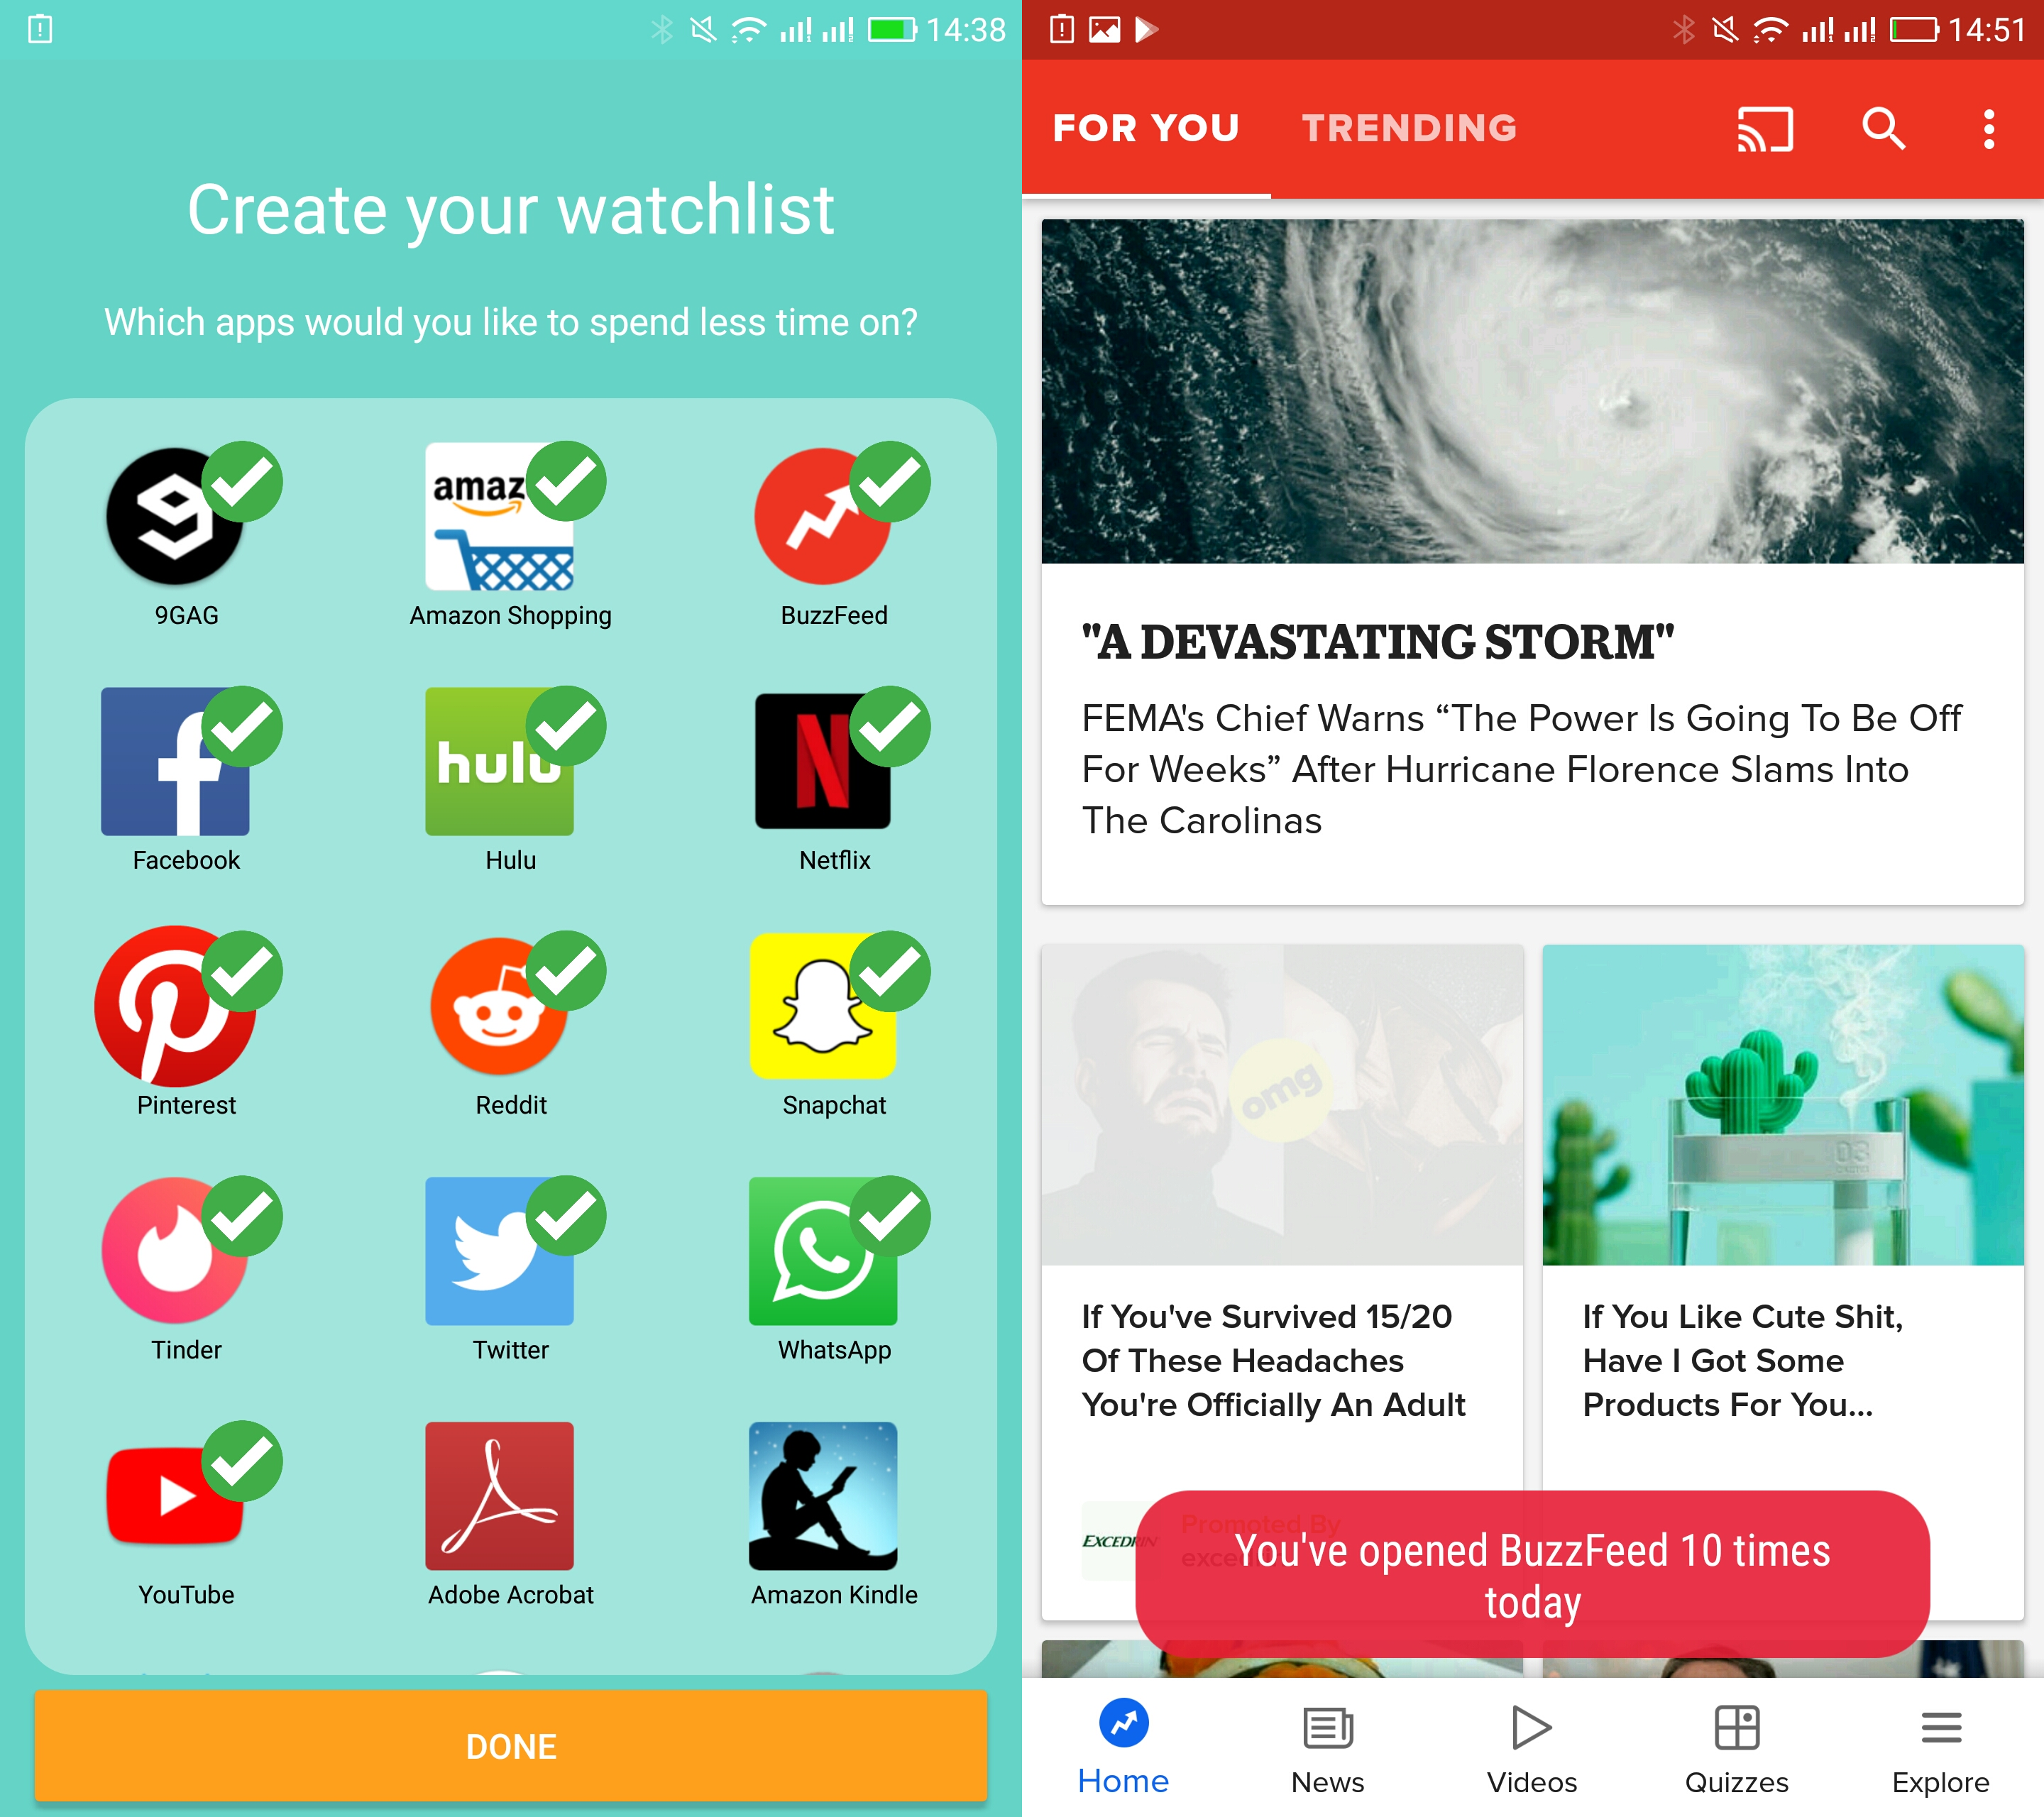
\includegraphics[width=\linewidth]{figures2/android_combined}
\caption{Screenshots from the mobile version of HabitLab.\\
Left: The goal selection screen, where users choose which apps to spend less time on.\\
Right: An example intervention, which shows the visit count when a user opens a goal app. %\msb{save space by cutting the image after the Iqiyi row. No point in having a nearly empty row at the bottom}
}
  \label{fig:android-goal-selection}
\end{figure}

% \begin{figure}
% \begin{minipage}[t]{0.49\linewidth}
% 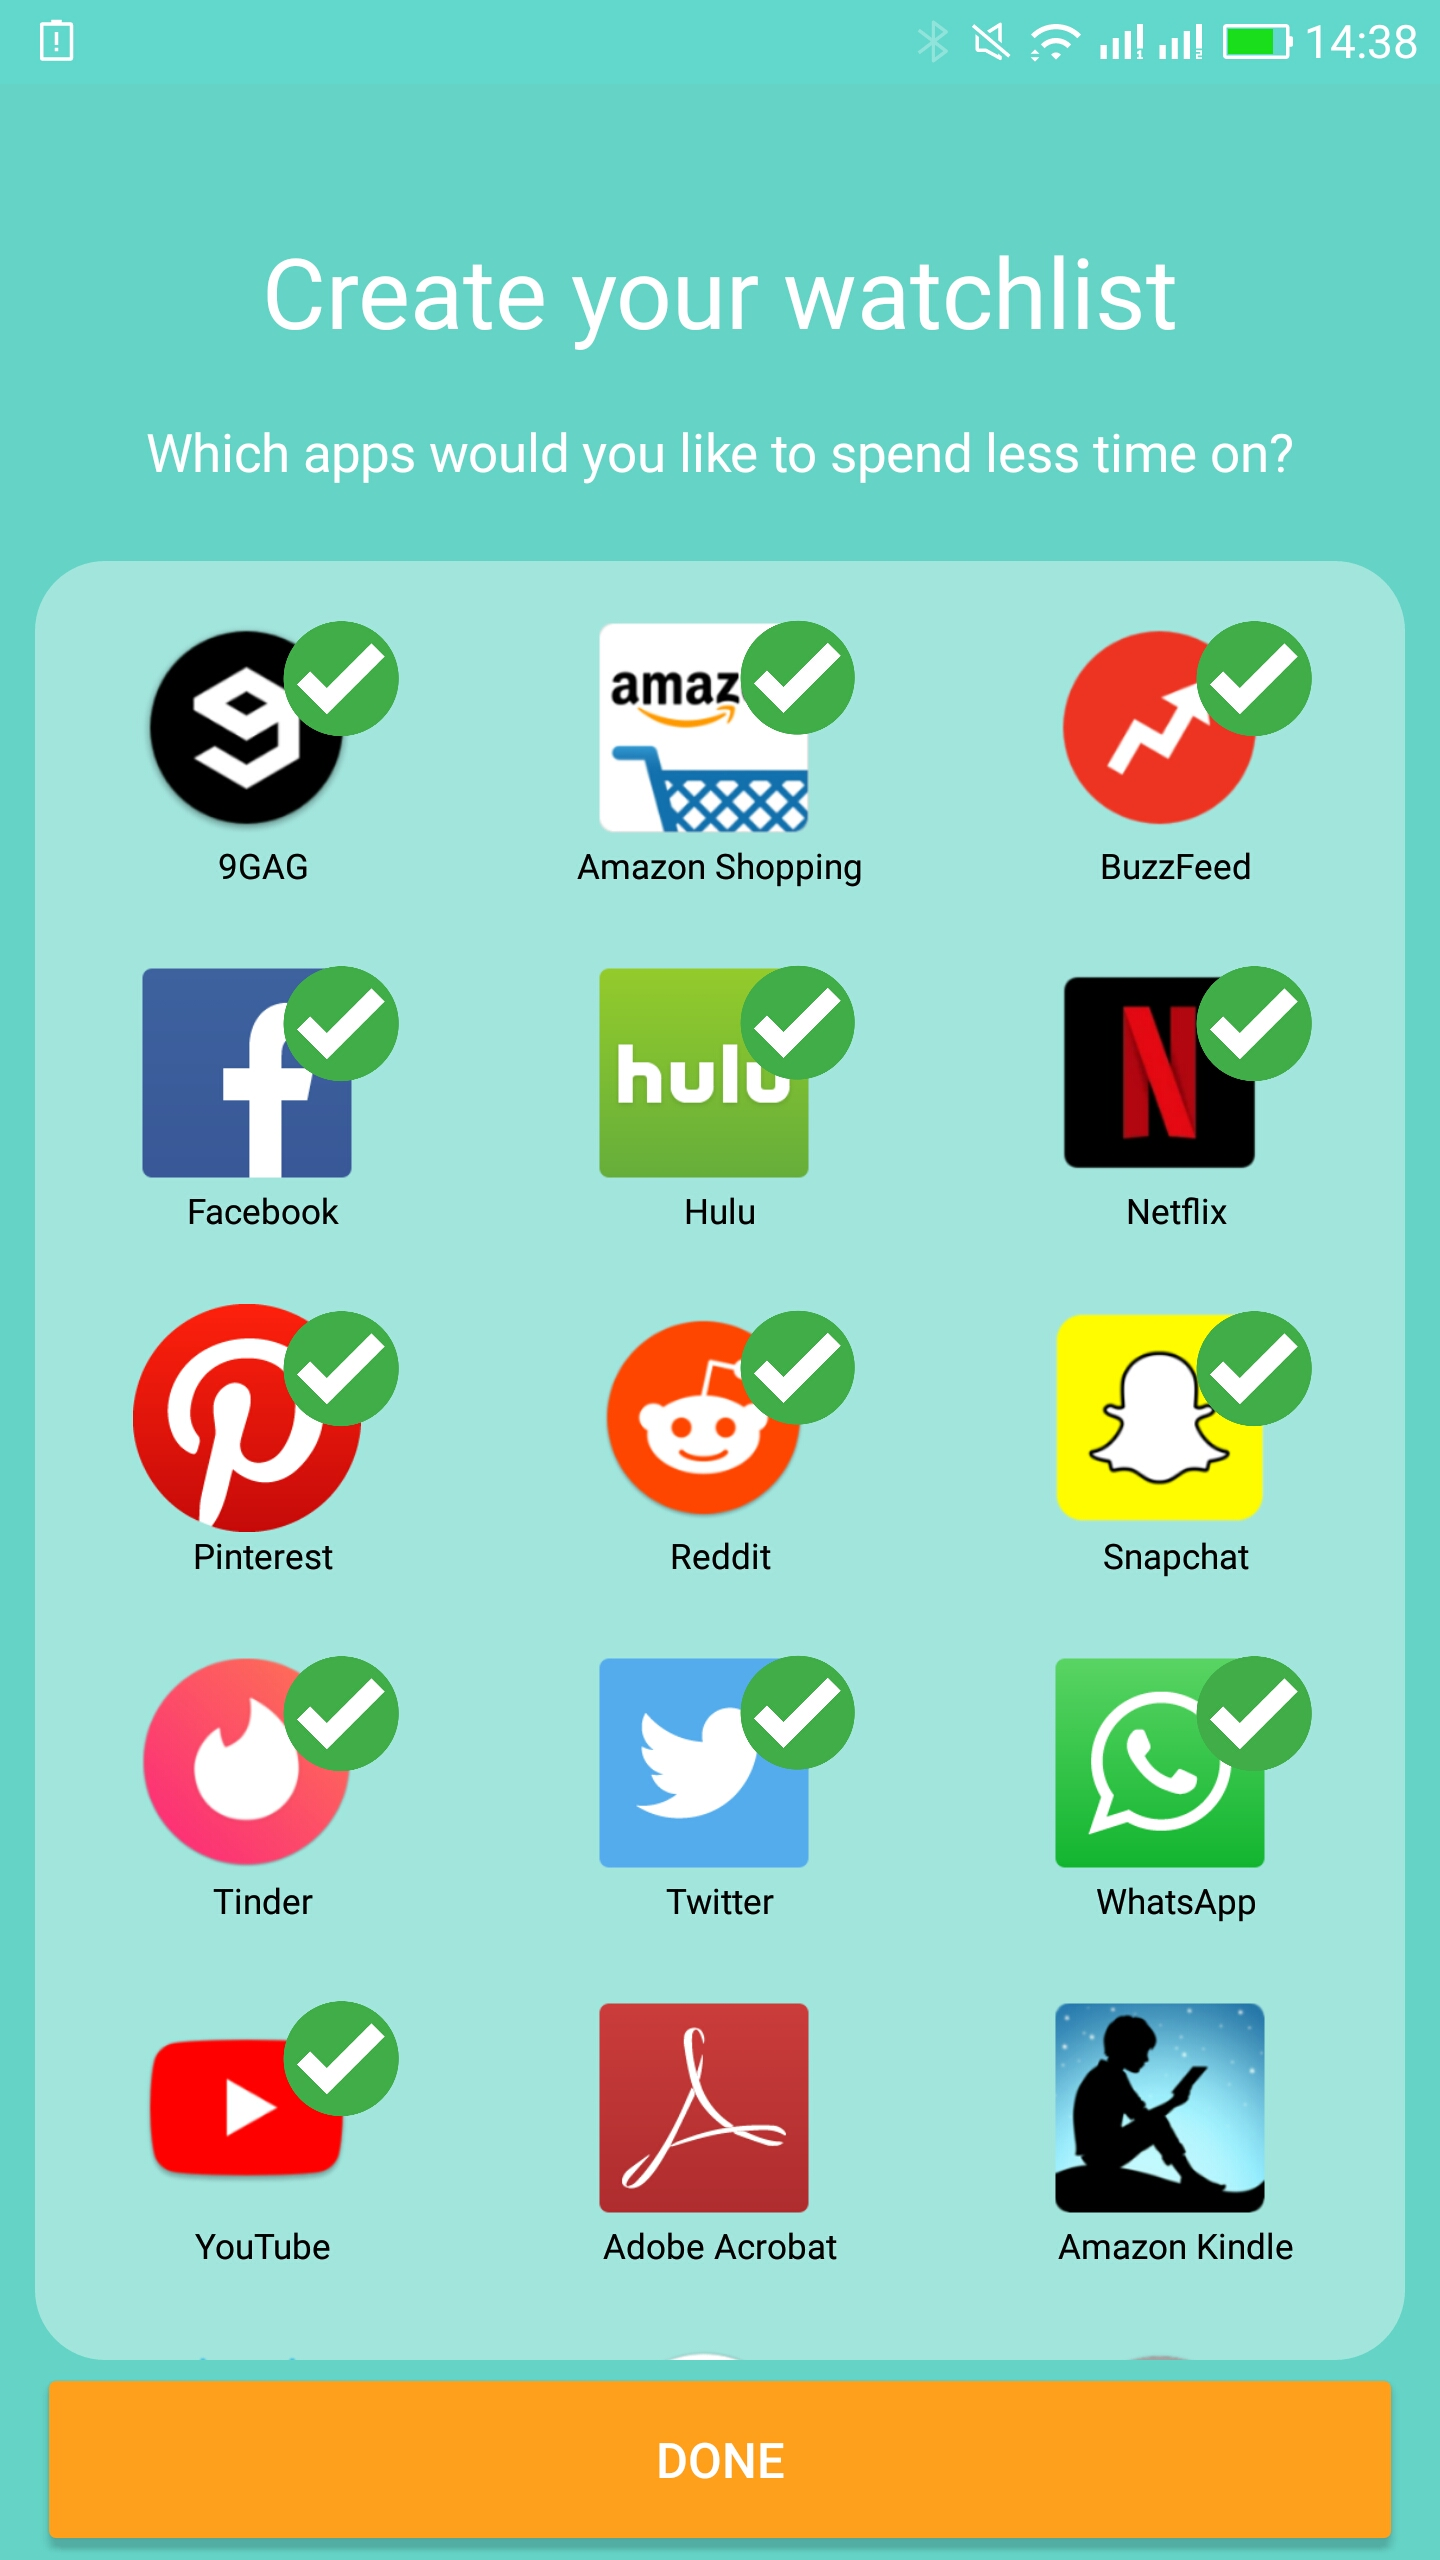
\includegraphics[width=\linewidth]{figures2/android-goal-selection}
% \caption{The goal selection screen, where users choose which apps to spend less time on (mobile version). %\msb{These two mini vertical figures are hard to read. Make it one figure with one caption underneath both.}
% }
%   \label{fig:android-goal-selection}
% \end{minipage}%
% \hfill
% \begin{minipage}[t]{0.49\linewidth}
% 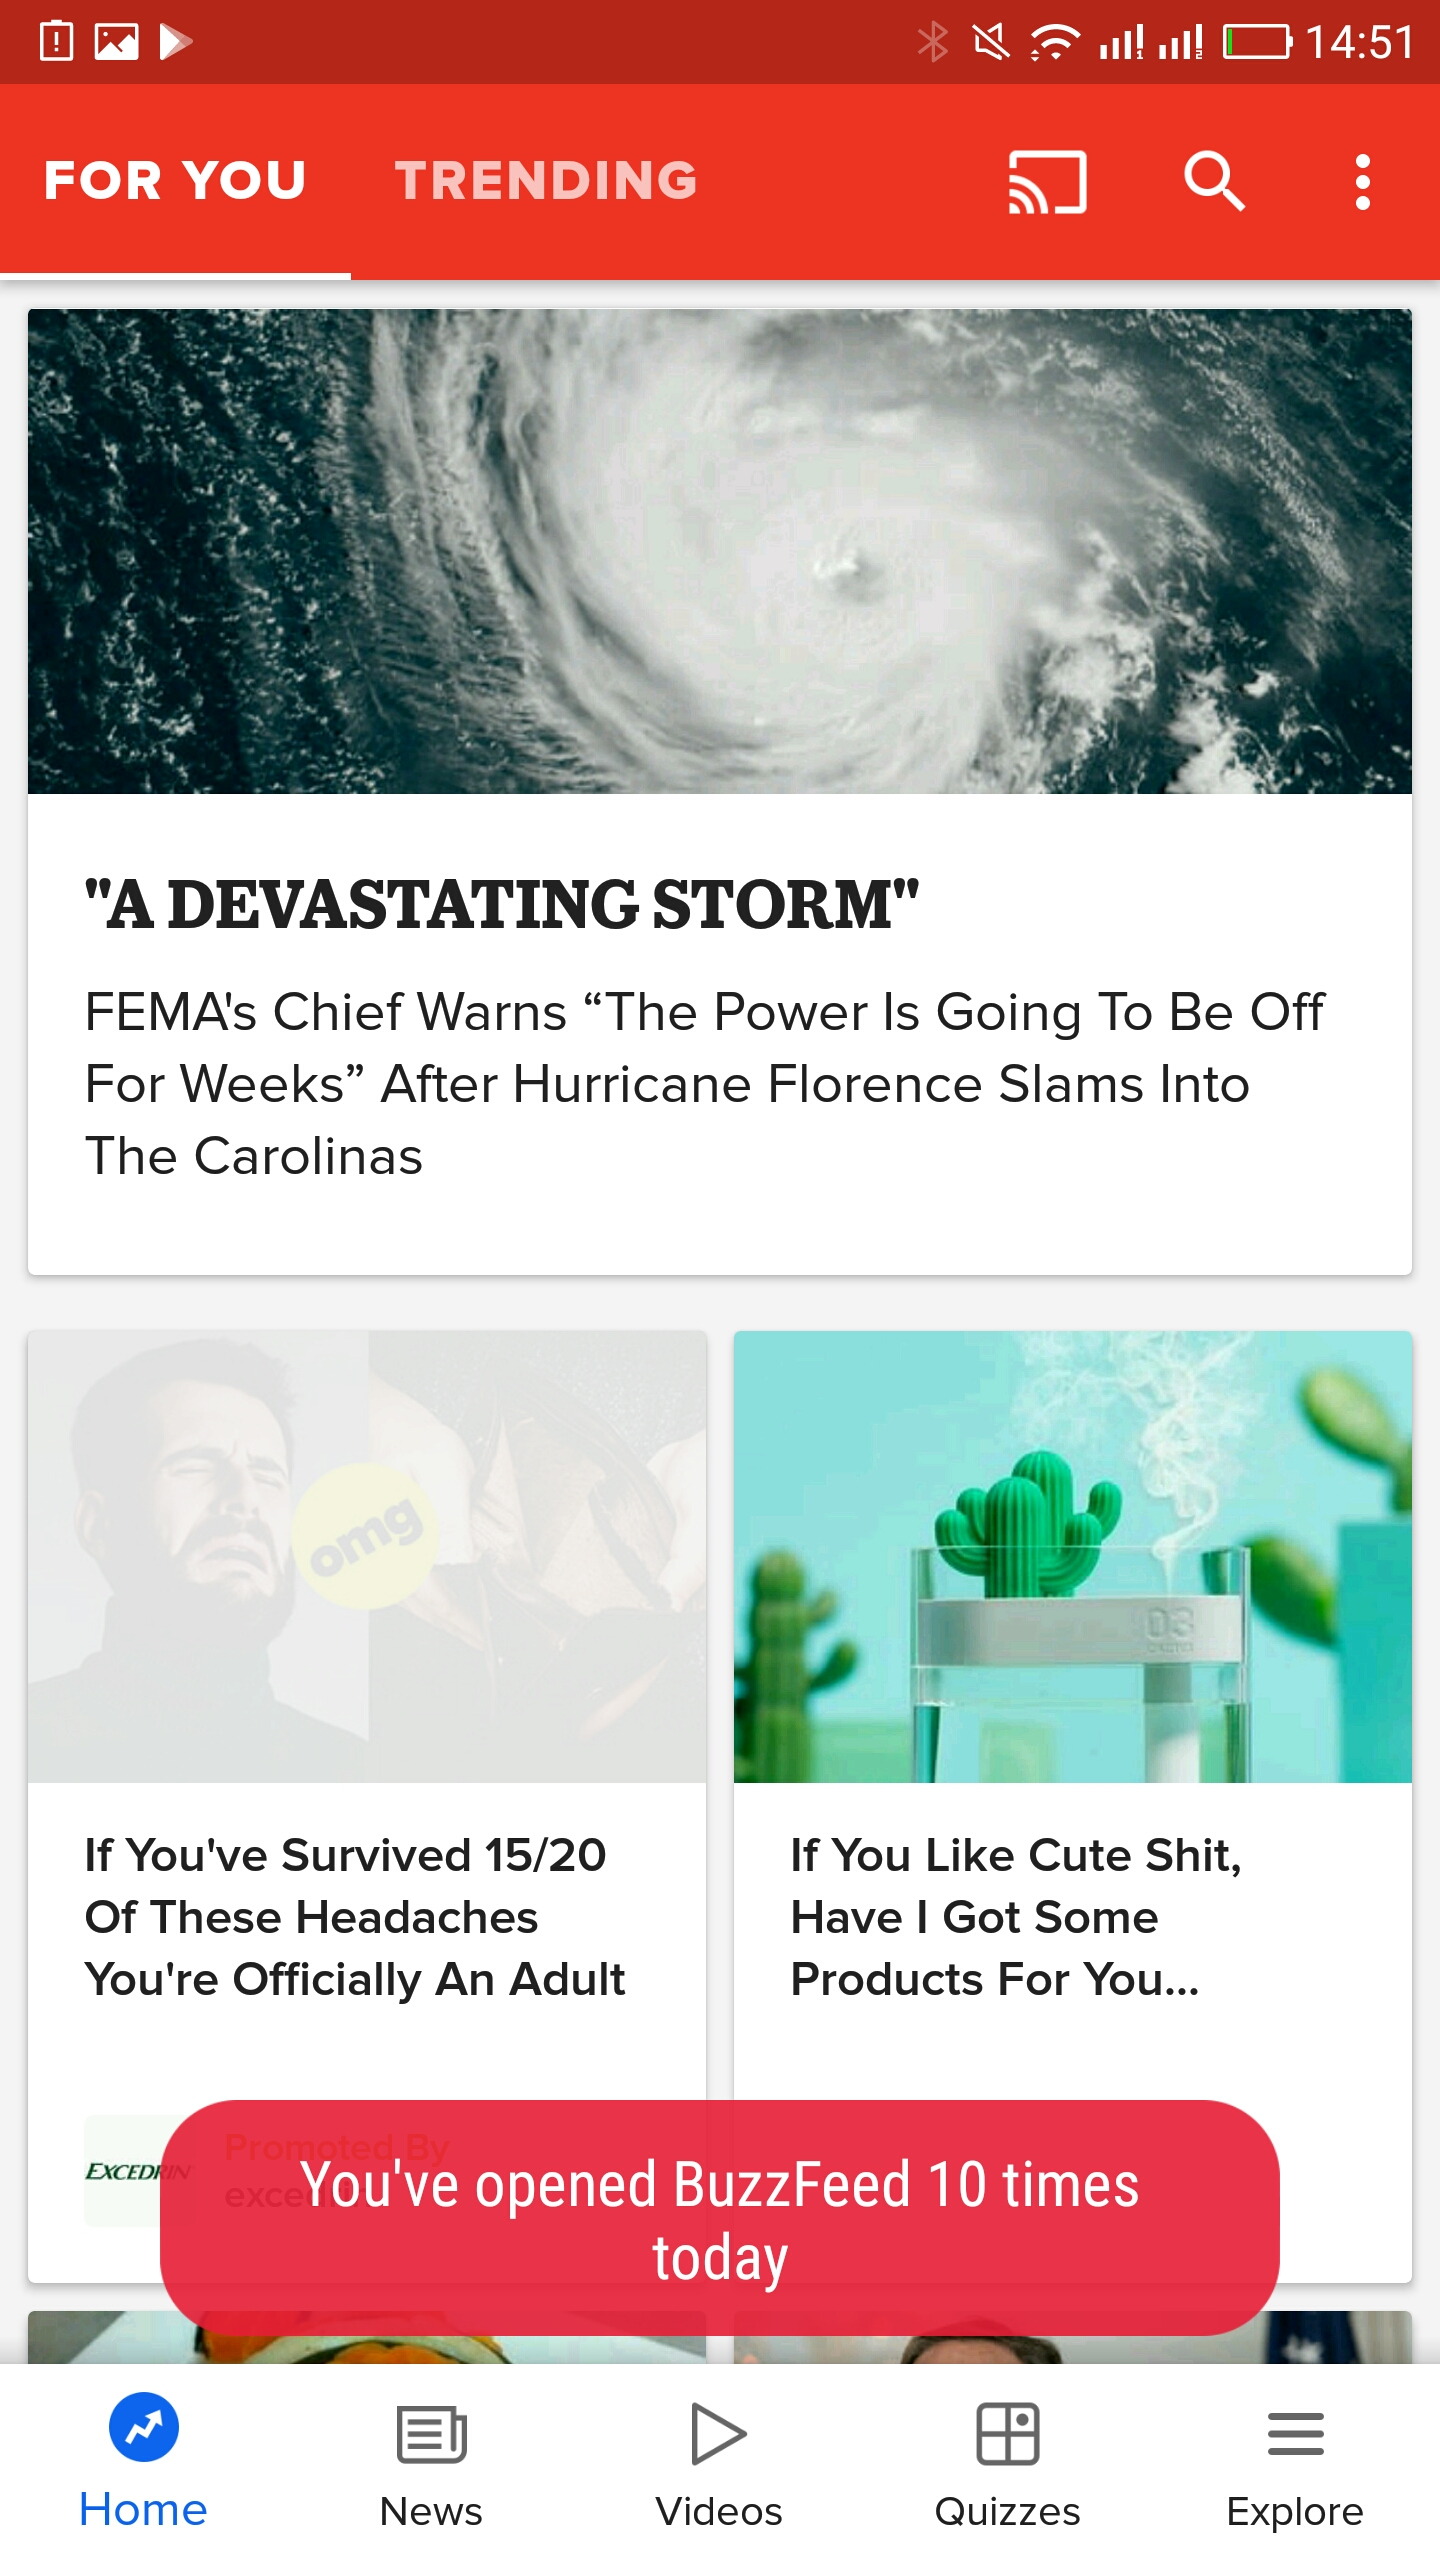
\includegraphics[width=\linewidth]{figures2/android-intervention}
% \caption{An example intervention, which shows the visit count when a user opens an app (mobile version).}
%   \label{fig:android-intervention}
% \end{minipage}
% \end{figure}

% \begin{figure}
% 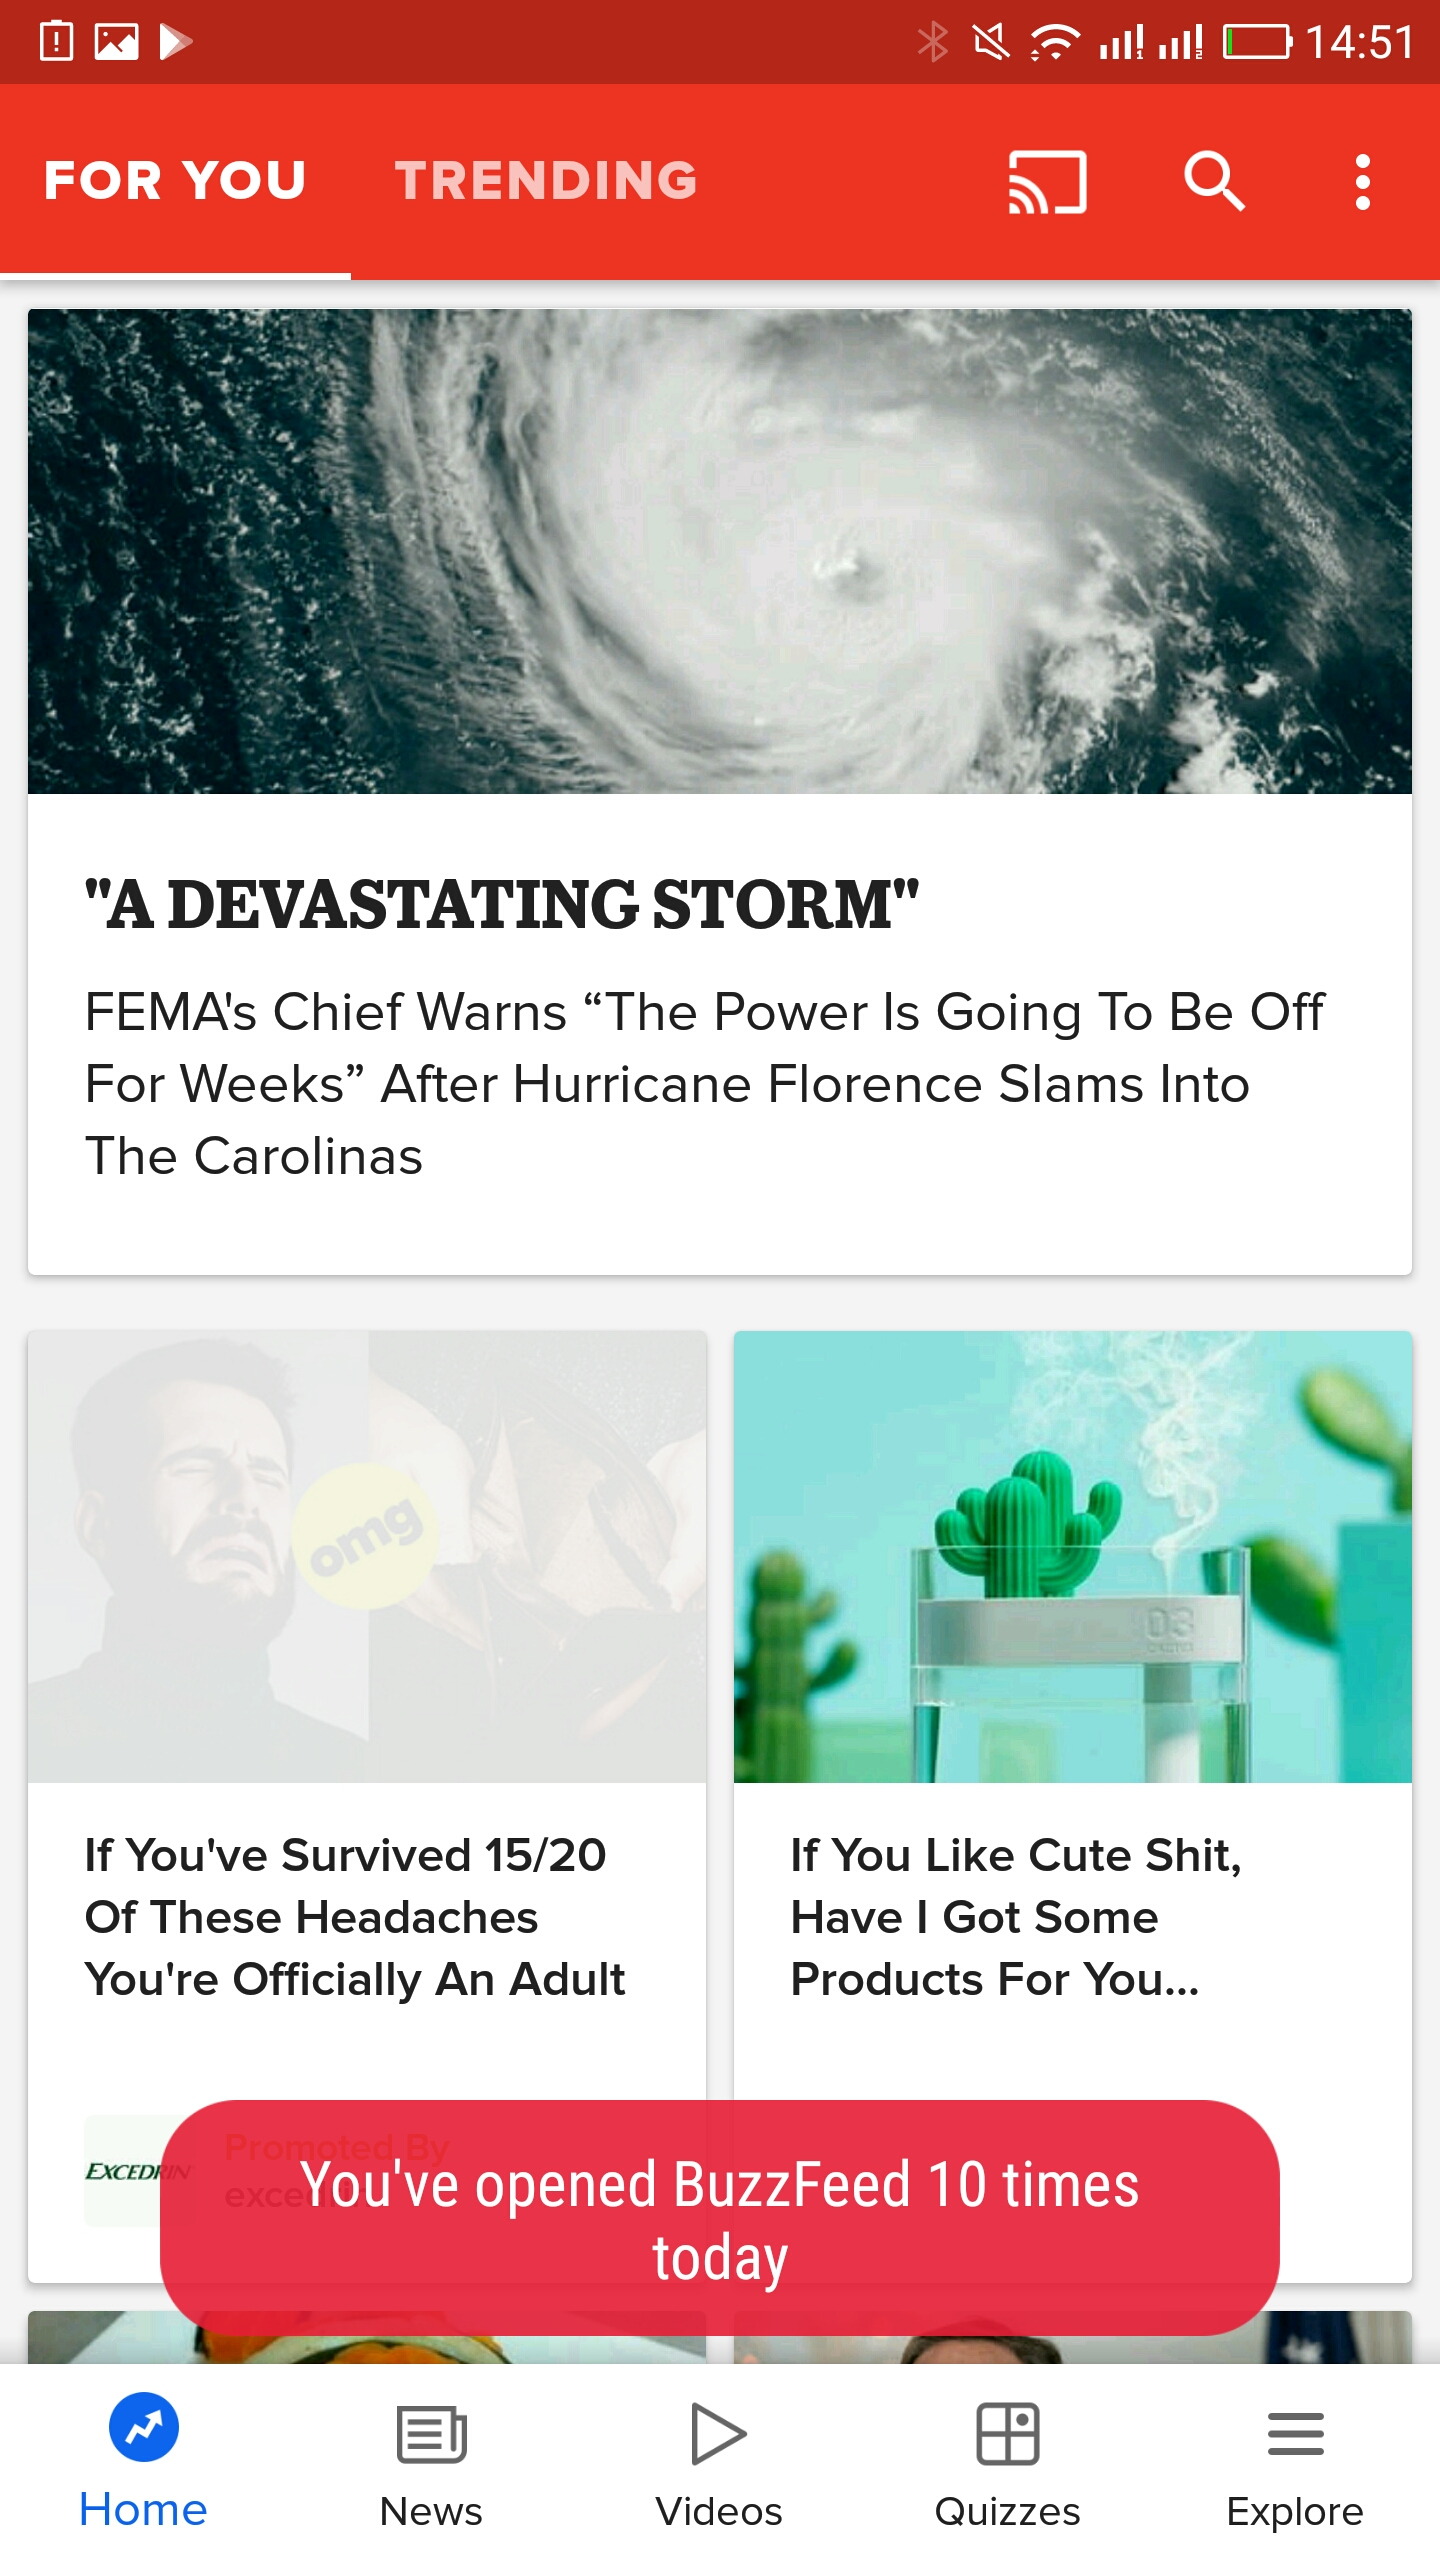
\includegraphics[width=\linewidth]{figures2/android-intervention}
% \caption{Mental model interface: each time the user sees a new intervention, HabitLab names it and explains about rotation.}
%   \label{fig:info}
% \hfill
% \includegraphics[width=\linewidth]{figures2/android-watchlist}
% \caption{User control interface: in addition to the mental model information, HabitLab gives users a direct interface to disable the new intervention.}
%   \label{fig:power}
% \end{figure}

\begin{figure}
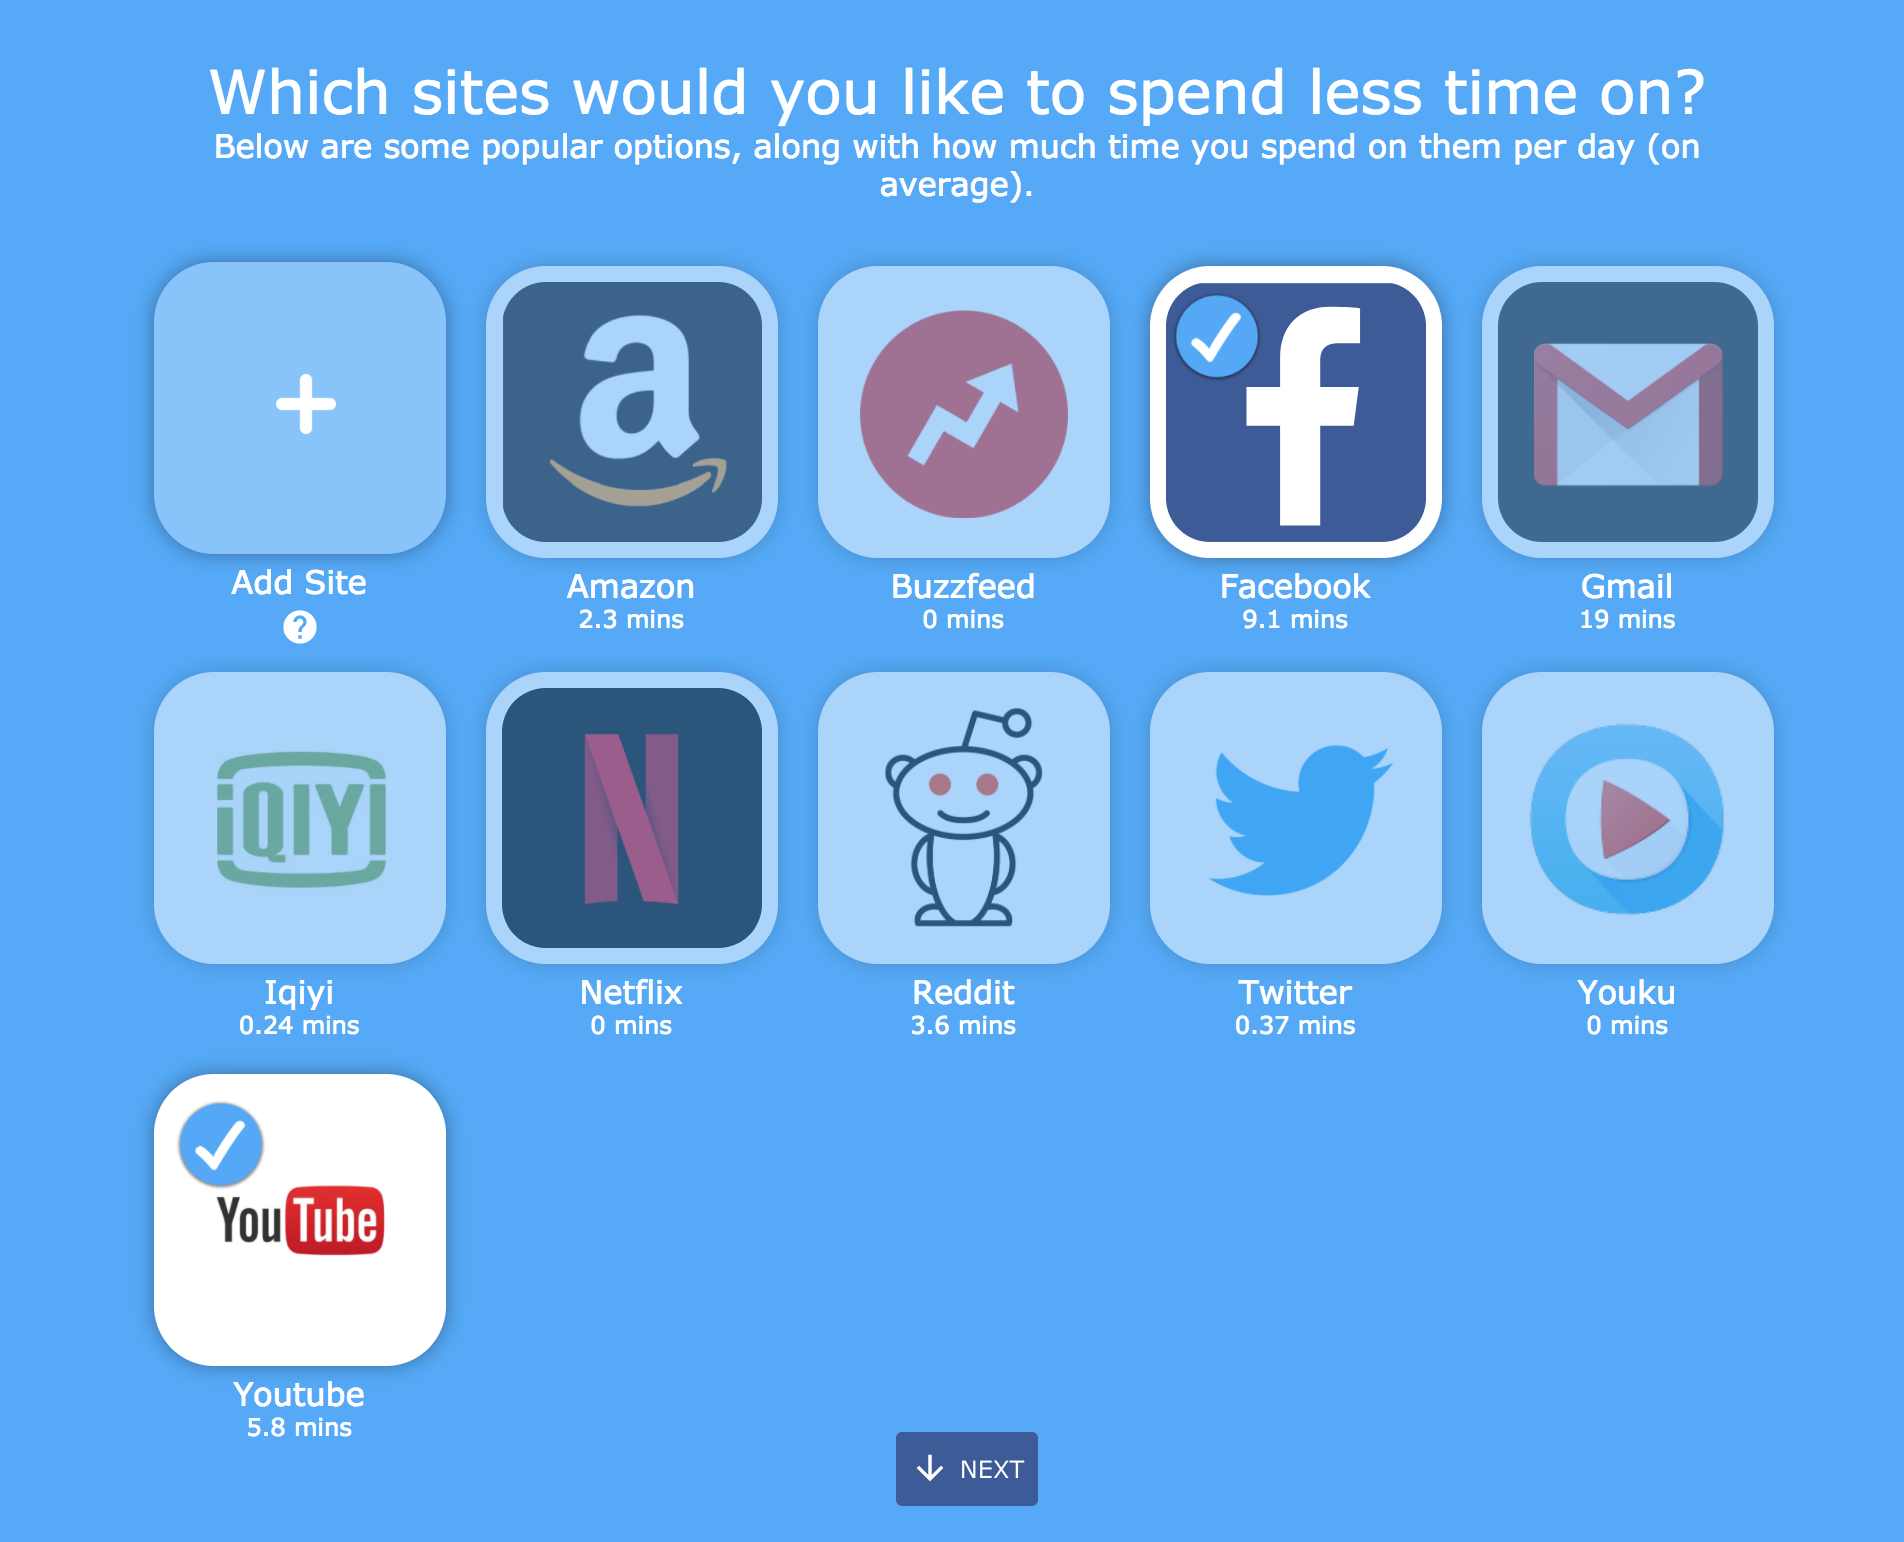
\includegraphics[width=\linewidth]{figures2/chrome-goal-selection}
\caption{The goal selection screen, where users choose which sites to spend less time on (browser version). %\msb{save space by cutting the image after the Iqiyi row. No point in having a nearly empty row at the bottom}
}
  \label{fig:chrome-goal-selection}
\end{figure}

\begin{figure}
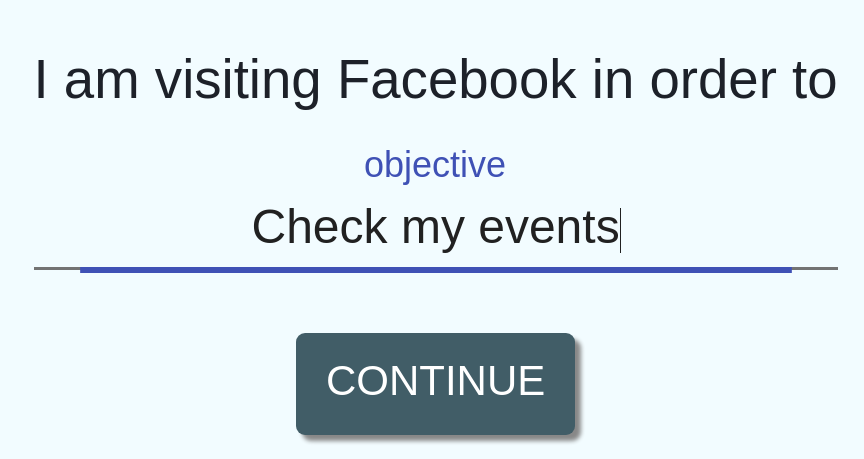
\includegraphics[width=\linewidth]{figures2/chrome-intervention-v3}
\caption{An example intervention, which asks a user to write their objective for visiting a site (browser version). %\msb{This page is really crowded with figures. I suggest moving one onto the next page.} 
% \msb{Save space by reducing this figure to start just above ``I am visiting FB to...''. The turn off button isn't necessary and it adds a ton of space to the paper.}
}
  \label{fig:chrome-intervention}
\end{figure}

There are two versions of HabitLab: a Chrome extension, and an Android app. Both follow the structure of allowing users to choose what they wish to spend less time on (setting goals), and deploying interventions to meet those goals. %The format of the goals differ between the two platforms.
On the Chrome version, users choose sites to spend less time on (goal sites -- for example, \url{facebook.com}), as shown in Figure~\ref{fig:chrome-goal-selection}. On Android, users choose particular apps to spend less time on (goal apps -- for example, the Facebook Android app), as shown in Figure~\ref{fig:android-goal-selection}. Interventions are deployed when users visit a goal site on Chrome (Figure~\ref{fig:chrome-intervention}), and when users open a goal app on Android, as shown in Figure~\ref{fig:android-goal-selection}.

%Particular interventions also differ between the platforms: the Chrome version includes a number of site-specific interventions such as a news feed remover for Facebook, whereas the Android version only has generic interventions that can be applied to all apps. The interventions are designed based on theories such as Cialdini's factors of influence~\cite{cialdini1987influence} and the behavior change wheel taxonomy of behavior change interventions~\cite{abraham2008taxonomy}. A complete list of interventions on the Chrome and Android versions along with descriptions can be found in the Appendix.

\subsection{Mobile and Browser version Differences}

The Chrome extension and Android app differ in some minor details. They support different sets of goals: users select apps to reduce time on in the Android version, whereas users choose sites to reduce time on in the Chrome version. Additionally, the specific set of interventions available differs between the platforms to fit the design languages of the browser and the mobile phone. The Chrome version has certain interventions which are site-specific -- such as a news feed remover that is specific to Facebook. However, because Android does not allow applications to edit each other's view trees, the Android version's interventions are all glass pane overlays, and thus are general and can be used on any app. The concept of a session is different on the platforms: in the Chrome version, a session is time on a site until that tab is either closed or the user goes to a different domain. Time measured is active time -- so if the tab is not focused, or if there is no keyboard or mouse activity for over a minute, the timer is temporarily paused. However, on Android, because there is no concept of a tab, the measurement of a session is different. There, a session is considered the duration over which an app is opened and focused. Closing the app, switching to a different app, or turning off the phone will end the current session.

%\subsection{Design of Interventions}

The design of HabitLab's interventions is based on theories such as Cialdini's factors of influence~\cite{cialdini1987influence} and the behavior change wheel taxonomy of behavior change interventions~\cite{abraham2008taxonomy}. Description of the interventions on the Chrome and Android versions can be found in the Appendix.



%\subsection{Userbase}

As of writing, the Chrome version has over 8000 daily active users, and the Android version has over 500 daily active users. The users were not explicitly recruited, but were rather all organic installs who discovered the extension/app via sources such as the Chrome/Play store, or were referred to it via press coverage in sources such as Wired or the New York Times.

